%%%%%%%%%% NO OLVIDAR COLOCAR ESTE COMENTARIO CON EL NUMERO DE EJERCICIO %%%%%%%%%%%%%
%%%%%%%%%%%%%%%%%%% EJERCICIO 6 %%%%%%
%%Text bf para negrilla , el \\ es para el salto de linea.
%%El primer \\ hace un espacio en el texto y el 2 \\ crea otro espacio
\textbf{Traslado períodos anticipados a períodos vencidos}\newline
El siguiente diagrama representa un traslado de períodos anticipados a períodos vencidos, sin afectar la serie.\\ \\

\textbf{Solución.}\\
\begin{center}

 \renewcommand{\arraystretch}{1.5}% Margenes de las celdas
 %Creación de la cuadricula
 \begin{longtable}{|c|c|c| }
  %Creamos una linea horizontal
  \hline
  %Definimos el color de la primera fila
  \rowcolor[HTML]{FFB183}
  %%%%% INICIO ASIGNACIÓN FECHA FOCAL %%%%%%%
  %%%%%%%%%% INICIO TITULO
  %Lo que se hace aquí es mezclar las 3 columnas en una sola
  \multicolumn{3}{|c|}{\cellcolor[HTML]{FFB183}\textbf{1. Asignación período focal}}                           \\ \hline
  %%%%%%%%%% FIN TITULO
  %%%%% INICIO DECLARACIÓN DE VARIABLES %%%%%%%
  \multicolumn{3}{|c|}{$pf : 0 pma$}                                                                         \\ \hline
  %Definimos el color de la primera fila
  \rowcolor[HTML]{FFB183}
  %%%%% INICIO DECLARACIÓN DE VARIABLES %%%%%%%
  %%%%%%%%%% INICIO TITULO
  \multicolumn{3}{|c|}{\cellcolor[HTML]{FFB183}\textbf{2. Declaración de variables}}                         \\ \hline
  %%%%%%%%%% FIN TITULO
  %%%%%%%%%% INICIO DE MATEMÁTICAS
  \multicolumn{1}{|c|}{\cellcolor[HTML]{FFB183}\textbf{Valores monetarios}}    & \multicolumn{1}{c|}{\cellcolor[HTML]{FFB183}\textbf{Valores no monetarios}} & \multicolumn{1}{c|}{\cellcolor[HTML]{FFB183}\textbf{Incógnitas}} \\ \hline
  R= 40.000 COP & $i=2,5\% pmv$ & VP = ? COP\\
  $P_{0}=$ 40.000 COP & $n={11}\ pmv$ & \\
  & $n_{0}=12 pmv$ & \\ \hline

  %%%%%%%%%% FIN DE MATEMÁTICAS
  %%%%% FIN DECLARACIÓN DE VARIABLES


  %%%%% INICIO FLUJO DE CAJA
  \rowcolor[HTML]{FFB183}
  \multicolumn{3}{|c|}{\cellcolor[HTML]{FFB183}\textbf{3. Diagrama de flujo de caja}}                        \\ \hline
  %Mezclamos 3 columnas y pondremos el dibujo
  %%%%%%%%%%%%% INSERCIÓN DE LA IMAGEN
  \multicolumn{3}{|c|}{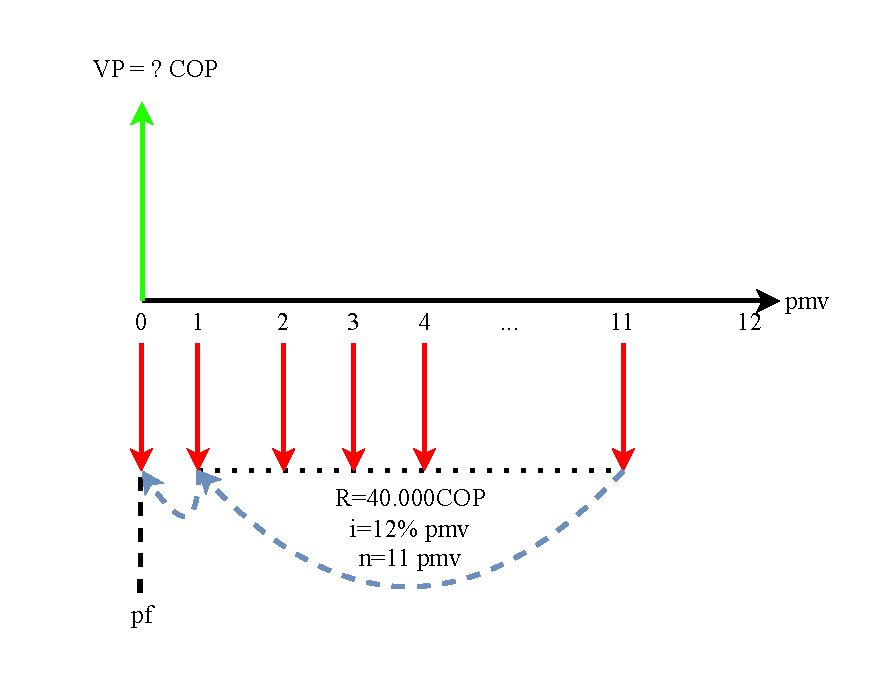
\includegraphics[width=0.95\columnwidth, trim=-3 -3 -3 -7]
  {4_Capitulo/img/ejemplos/Exportados/Ejemplo.pdf }} \\ \hline
  %%%%%%%%%%%%% FIN INSERCIÓN DE IMAGEN
  %%%%%FIN FLUJO DE CAJA



  %%%%% INICIO DECLARACIÓN FORMULAS
  %%%%%%%%%%% INICIO TITULO
  \rowcolor[HTML]{FFB183}
  \multicolumn{3}{|c|}{\cellcolor[HTML]{FFB183}\textbf{4. Declaración de fórmulas}}                          \\ \hline
  %%%%%%%%%%% FIN TITULO
  %%%%%%%%%%% INICIO MATEMÁTICAS
  \multicolumn{3}{|c|}{VP=R$\frac{(1-(1+i)^{-n})}{i}$ \hspace{35pt}{Valor presente serie uniforme vencida}}    \\ \hline                                       
  \multicolumn{3}{|c|}{\cellcolor[HTML]{FFB183}\textbf{5. Desarrollo matemático}}                            \\ \hline
  %%%%%%%%%% FIN TITULO
  %%%%%%%%%% INICIO MATEMÁTICAS
  \multicolumn{3}{|c|}{  $VP_{1}=$ 40.000 COP $\frac{1-(1+0,025)^{-11}}{0,025}$}\\
  \multicolumn{3}{|c|}{  $VP_{1}=$ 380.568,35 COP}\\
  \multicolumn{3}{|c|}{  $VP=VP_{1}+P_{0}$}\\
  \multicolumn{3}{|c|}{  $VP=$ 380.568,35 COP + 40.000 COP}\\ 
  \multicolumn{3}{|c|}{  $VP=$ COP 420.568,35 COP}\\ \hline
  %%%%%%%%%% FIN MATEMÁTICAS
  %%%%%% FIN DESARROLLO MATEMÁTICO

  \rowcolor[HTML]{FFB183}
  \multicolumn{3}{|c|}{\cellcolor[HTML]{FFB183}\textbf{6. Respuesta}}                                        \\ \hline

  \multicolumn{3}{|c|}{El valor del pago unico será de 420.568 COP}   \\ \hline
  
 \end{longtable}
 %Se crean dos lineas en blanco para que no quede el siguiente texto tan pegado
 %\newline \newline
\end{center}
%%%%%%%%%%%%%%%%%%%%%%%%%%FIN EJERCICIO 6 %%%%%%%%%%%%%%%%%%%%%%%%%%%